\section{Effect of Grid Storage} \label{sec:res-storage}

Having implemented the stencils using the various grid access strategies, we then went on to explore optimization possibilities in the grid storage, namely how the neighborship tables could be stored in a way to enable faster accesses. The different approaches are described in section \ref{sec:grid-implementations}. We evaluated four different neighborship table structures, resulting from the combinations of the following two properties: First, the depth of the neighborship table, i.e. whether only neighbors (\emph{chasing} variant) or also neighbors-of-neighbors (\emph{non-chasing} variant) were stored. Second, whether the neighborship table was \emph{compressed} or \emph{uncompressed}.

\begin{figure}
    % ax=u.barplot(df64mins[(df64mins["stencil"]=="hdiff")&df64mins["z-curves"]&(df64mins["size-x"]>=128)], grp=u.col.stencil+u.col.size, cat=u.col.storage, tickrot=0, y="rel")
    % ax.set_ylim(bottom=1)
    % fig=u.plotdone()
    % u.plotsave("report/img/hdiff-z-curves-sizes-storage.pdf", fig)
    \comment{
          stencil  size-x  size-y  size-z  unstructured        variant  z-curves  no-chase   comp  threads-x  threads-y  threads-z       min       max       avg    median
    11327   hdiff     128     128      64          True         idxvar      True     False  False         64          1          8   50000.0   53000.0   51000.0   51000.0
    12079   hdiff     128     128      64          True         idxvar      True     False   True         32          1         16   52000.0   56000.0   53000.0   53000.0
    10516   hdiff     128     128      64          True         idxvar      True      True  False         32          2          8   47000.0   50000.0   48000.0   49000.0
    10880   hdiff     128     128      64          True          naive      True      True   True         32          1          8   48000.0   51000.0   50000.0   50000.0
    32073   hdiff     512     512      64          True         idxvar      True     False  False         64          1          8  801000.0  828000.0  817000.0  820000.0
    31623   hdiff     512     512      64          True         idxvar      True     False   True        128          1          2  734000.0  746000.0  741000.0  741000.0
    32178   hdiff     512     512      64          True  idxvar-shared      True      True  False         32          1         16  819000.0  854000.0  838000.0  841000.0
    31541   hdiff     512     512      64          True          naive      True      True   True        128          1          2  707000.0  721000.0  713000.0  710000.0
    }
	\begin{center}
    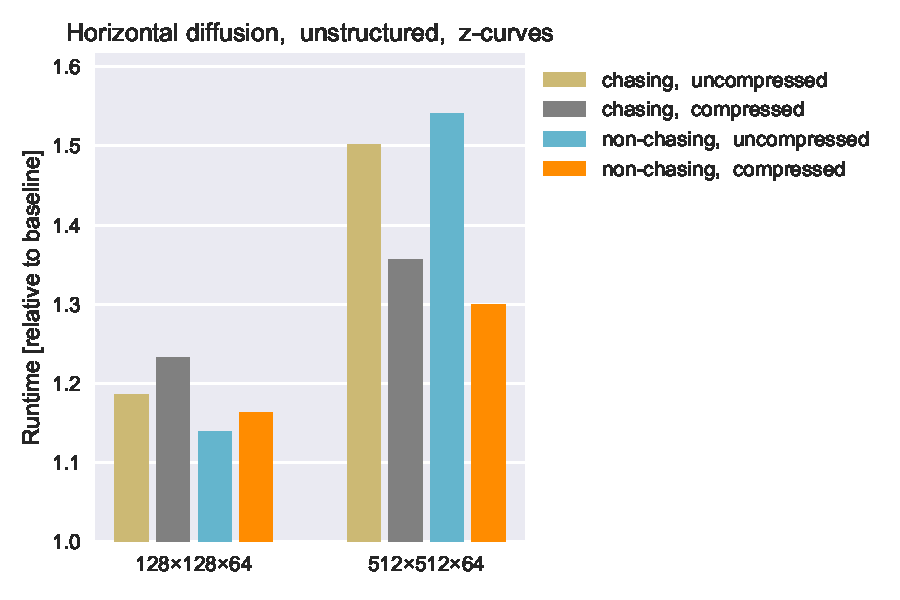
\includegraphics[scale=0.75]{hdiff-z-curves-sizes-storage.pdf}
	\end{center}
    \caption{\label{fig:hdiff-sizes-storage} Effect of neighborship table properties on runtime depending on problem size. This shows the slowdowns relative to the fastest regular grid implementations for the \emph{hdiff} stencil on a small and a large grid (both \emph{z-curves} memory layout with \emph{double} precision). The respective fastest access variant is plotted for each bar, which is one of \emph{idxvar}, \emph{naive}, and \emph{shared} for the shown benchmarks. This example for the \emph{hdiff} stencil is representative of the other two benchmarks as well, where the slowdowns follow a similar pattern. (Note that in the \emph{fastwaves} stencil, pointer chasing is not applicable as there only direct neighbors are accessed.) Baseline: fastest regular grid implementation.}
\end{figure}

\subsection{Pointer Chasing vs. Neighbor-of-Neighbor Storage}
\label{sec:results-chasing}

\begin{table}
    %chase-v-no-chase.txt
	\begin{center}
    \begin{tabular}{l c p{1.5cm} p{1.5cm} p{2.5cm} l}
        \hline
        \textbf{Size} & \textbf{Chasing?} & \textbf{\texttt{tex\_\allowbreak cache\_\allowbreak hit\_\allowbreak rate}} & \textbf{\texttt{l2\_\allowbreak tex\_\allowbreak hit\_\allowbreak rate}} & \textbf{\texttt{stall\_\allowbreak memory\_\allowbreak dependency}} & \textbf{Runtime} \\
        \hline
        \hline
        $128\times 128\times 64$ & \checkmark &             $73\%$ & $68\%$ & $59\%$ & $41 \mu s$ \\
        $128\times 128\times 64$ & - & $67\%$ & $72\%$ & $54\%$ & $40 \mu s$ \\
        \hline
        $512\times 512\times 64$ & \checkmark &             $68\%$ & $684\%$ & $74\%$ & $841 \mu s$ \\
        $512\times 512\times 64$ & - & $63\%$ & $37\%$ & $60\%$ & $1042 \mu s$ \\
        \hline
    \end{tabular}
	\end{center}
    \caption{\label{tab:chasing} Selected metrics, including L1 cache hit rate (\texttt{tex\_\allowbreak cache\_\allowbreak hit\_\allowbreak rate}), for runs of the \emph{laplap} stencil on unstructured grids of different sizes (all of them in \emph{z-curves} memory layout with \emph{double} precision, \emph{uncompressed} neighborship table), both with and without pointer chasing. The \emph{idxvar} access strategy was used with a fixed launch configuration of $64\times 4\times 2$ threads.}
\end{table}

Two of the three benchmarked stencils, \emph{Laplace-of-Laplace} and \emph{horizontal diffusion}, access neighbors beyond the directly face-touching cells (neighbors-of-neighbors). For those stencils, we first assessed the performance when only direct neighbors are explicitly stored. This approach requires \emph{pointer chasing}: To access the neighbor of a neighbor, two sequential lookups to the neighborship table become necessary. As the second lookup can only be started once the first one has completed, a higher latency  occurs in this variant. Therefore, we then also tested variants in which the neighbors-of-neighbors were explicitly stored in memory, reducing the number of required memory lookups for these types of accesses from two to one. We call this \emph{non-chasing} neighborship storage. This approach comes at the cost of a higher memory footprint.

Generally, we observed the following trend: If the grid is small or compressed, pointer chasing becomes an issue, and thus the \emph{non-chasing} variants provide an advantage. In larger \emph{uncompressed} grids, the latency of the two lookups required for neighbors-of-neighbor access can be effectively hidden. This is visible in figure \ref{fig:hdiff-sizes-storage}, which outlines the differences of the storage approaches for the fastest respective variant of the \emph{hdiff} stencil on grids of different sizes. 

In all cases, a higher total number of device memory and L2 cache reads was observed for the \emph{non-chasing} variants. This is to be expected, as \emph{non-chasing} variants need to store and read more information from a larger number of different addresses. When pointers to neighbors-of-neighbors are explicitly stored, the L1 cache hit rate lowers by around $6\%$ in both large and small grids. In large grids, the L2 cache hit rate also drops dramatically; for smaller grids, it remains unaffected.

In large \emph{non-chasing} grids, the additional neighbor-of-neighbor entries affect cache locality more negatively than in small grids. This is because larger grids have more neighborship table entries, while the cache size remains constant -- consequently, some data has to be evicted from the cache. This does not happen as often in a smaller grid. The variants that perform pointer chasing experience a higher percentage of stalls caused by memory dependencies; neighbor-of-neighbor reads block progress as the second lookup waits for the result of the first one. 

We conclude that non-chasing storage is beneficial to small grids, where it is effective in reducing latency, and unfavorable for larger grids due to the caused cache evictions (especially in the L2 cache) increasing the latency of neighbor accesses. Table \ref{tab:chasing} shows an overview of the metrics discussed in this paragraph for an exemplary stencil run.

\subsection{Effect of Neighborship Table Compression}
\label{sec:results-comp}

As most unstructured grids have irregularities only in few places, much of the information in the neighborship tables is redundant. Moving forward, we wanted to investigate whether this redundancy could be made use of to further reduce unstructured stencil runtimes. In section \ref{sec:compression}, we described a very simple compression scheme for the neighborship tables motivated by this idea. In this section, we elaborate on its performance implications.

Using \emph{compressed} neighborship tables, we saw a reduction in runtimes  for most benchmarks on large $512\times 512\times 64$-sized grids. The highest relative speedups were attained for the \emph{laplap} stencil, which ran $23\%$ faster. In the \emph{hdiff} stencil, we achieved a speedup of $21\%$. In contrast, the \emph{fastwaves} stencil was slightly slowed down by the added overhead of compression and ran $3\%$ slower.

In smaller grids ($128\times 128\times 64$ and $64\times 64\times 64$), the additional level of indirection introduced by our compression scheme also mostly led to a deterioration in run times. The interplay of grid size and compression can also be seen in figure \ref{fig:hdiff-sizes-storage}.

In the following two subsections we will further elaborate on the efficacy of our compression scheme in terms of (reduced) memory requirements and detail the effects on parallel execution in an attempt to explain the observed runtimes.

\subsubsection{Distribution of Neighborship Table Entries After Compression}

\begin{table}
	\begin{center}
    \begin{tabular}{l l l l l l}
        \hline
        \textbf{Compressed?} & \textbf{Chasing?} & \textbf{Storage} & \textbf{\# Entries} & \textbf{Ratio\textsuperscript{*}} & \textbf{Freq.\textsuperscript{\dag}} \\
        \hline
        \hline
        - & \checkmark & both & $1,048,576$ & $1$ & $<1\%$\\
        - & - & both & $3,145,728$ & $1$ & $<1\%$\\
        \checkmark & \checkmark & row-major & $2054$ & $0.00078$ & $97.7\%$ \\
        \checkmark & \checkmark & z-curves & $2435$ & $0.00093$ & $20.3\%$ \\
        \checkmark & - & row-major & $4093$ & $0.00156$ & $96.9\%$ \\
        \checkmark & - & z-curves & $5299$ & $0.00202$ & $8.1\%$ \\
        \hline
    \end{tabular}
	\end{center}
	\textsuperscript{*}Ratio of number of compressed neighborship table entries to number of uncompressed neighborship table entries. \textsuperscript{\dag}Frequency of the most common entry in the neighborship table. 
    \caption{\label{tab:compression} Properties of neighborship table before and after compression for $512\times 512\times 64$-sized grids with different memory layouts (\emph{z-curves} and \emph{row-major}), for both \emph{chasing} and \emph{non-chasing} implementations. }
\end{table}

\begin{figure}
	\begin{center}
		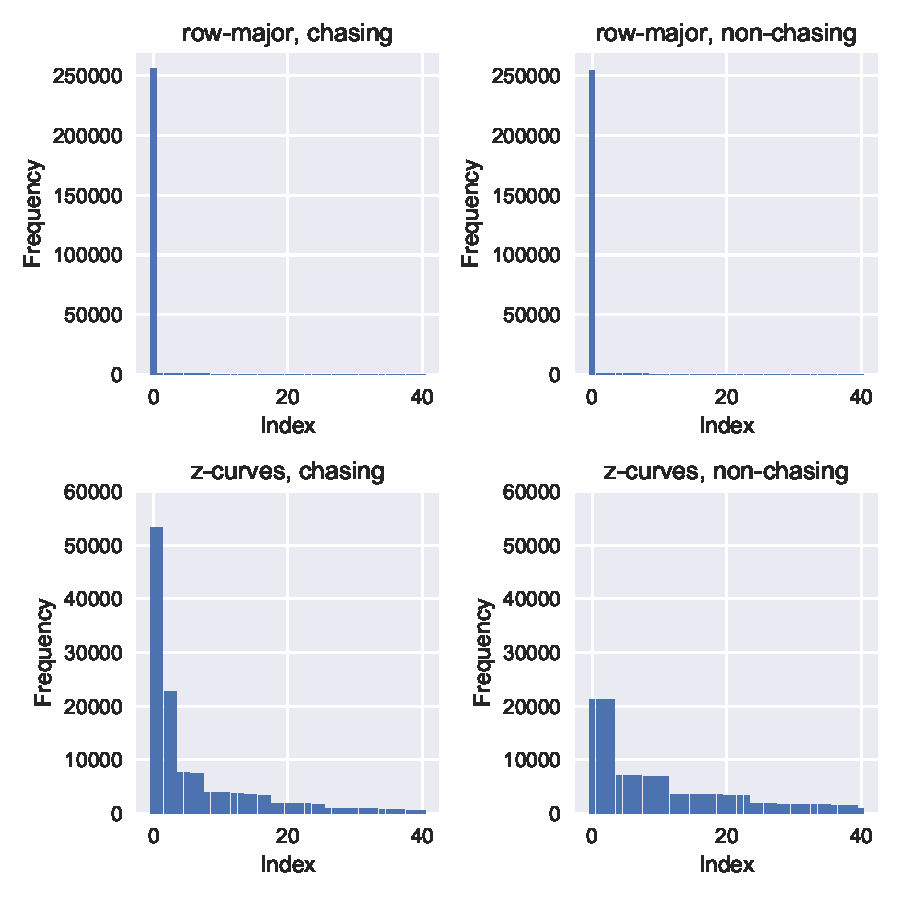
\includegraphics[scale=0.75]{dist-scaled.pdf}
		\caption{\label{fig:comp-dist} Distribution of the first 40 neighborship table entries of a $512\times 512\times 64$-sized grid for both benchmarked memory layouts and \emph{chasing} and \emph{non-chasing} implementations. The y-axis shows how many cells share the same relative neighborship offsets. The x-axis is the index in the neighborship table. A sharper peak means more effective compression. As an example, the first two entries in the \emph{chasing} neighborship table of a grid with \emph{z-curves} memory layout are shared by $53340$ cells. Compare this to the uncompressed case (not plotted), where each entry is shared across Z-levels between cells with equal X- and Y-coordinates, i.e. $64$ times in this example. \emph{Note the different scale in the bottom row!}}
	\end{center}
\end{figure}

Using the compression scheme, cells with the same neighbor \emph{patterns} can share neighborship table entries. Table \ref{tab:compression} and figure \ref{fig:comp-dist} show the distribution of unique patterns on a $512\times 512\times 64$-sized grid for the two memory layouts benchmarked (\emph{row-major}, \emph{z-curves}). In \emph{row-major} grids, the number of distinct patterns is lowest. In this case, only the elements in the halo have different neighborship pointers; all others share the top entry. Using a \emph{z-curves} layout, the distribution of neighborship table accesses is flatter. However, there is still a fairly high concentration of several frequently occurring patterns.

Note that a completely random grid would result in a very even distribution. In such a scenario, compression would not be able to reduce the number of entries meaningfully. 

\subsubsection{Runtime Effects of Compression on Stencil Execution} 

The motivating idea behind implementing compression for the neighborship tables was an anticipated improvement to the caching of frequently used neighborship table entries. As we observed, neighborship information is distributed favorably and concentrates around a few frequently used entries (see table \ref{tab:compression} in the previous section). By using compression, we hoped that these entries remain in the L1 cache, and thus reduce the number of expensive reads to the L2 cache (or even device memory) required for neighborship index lookups. Yet, because cells with identical neighborship patterns share neighborship table entries in the compressed scheme, a mapping from cell index to pattern index must be implemented. This mapping introduces an additional lookup, whose latency may offset the advantage of cached neighborship table entries.

\begin{table}
    \makebox[\textwidth][c]{
    \begin{tabular}{l c p{2cm} p{2cm} p{2cm} p{2cm} l}
        \hline
        \textbf{Size} & \textbf{Comp.?} & \textbf{\texttt{tex\_\allowbreak cache\_\allowbreak transactions}} & \textbf{\texttt{l2\_\allowbreak tex\_\allowbreak read\_\allowbreak transactions}} & \textbf{\texttt{dram\_\allowbreak read\_\allowbreak transactions}} & \textbf{\texttt{gld\_\allowbreak efficiency}} & \textbf{Runtime} \\
        \hline
        $64\times64\times64$   & -            &    $466,815$ &    $273,384$ &     $57,658$ & $85\%$ & $\mathbf{18\mu s}$ \\ 
	    $64\times64\times64$   & $\checkmark$ &    $\mathbf{528,064}$ &    $415,834$ &     $51,676$ & $74\%$ & $  19\mu s$ \\
        \hline                   
        $128\times128\times64$ & -            &  $1,925,279$ &  $1,468,085$ &    $508,748$ & $87\%$ & $\mathbf{51\mu s}$ \\
	    $128\times128\times64$ & $\checkmark$ &  $\mathbf{2,071,128}$ &  $1,420,441$ &    $508,208$ & $75\%$ & $  53\mu s$ \\
        \hline                   
        $512\times512\times64$ & -            & $29,980,144$ & $22,391,916$ &  $9,392,553$ & $91\%$ & $ 820\mu s$ \\
	    $512\times512\times64$ & $\checkmark$ & $\mathbf{31,760,437}$ & $20,805,522$ &  $9,402,833$ & $77\%$ & $ \mathbf{741\mu s}$ \\
        
        \hline
        %\\
        \hline
    \end{tabular}
    }
	\caption{\label{tab:comp-runtime} Runtimes and relevant metrics comparing executions of \emph{hdiff} stencil on \emph{compressed} and \emph{uncompressed} grids (\emph{z-curves} memory layout with \emph{double} precision, \emph{chasing} neighborship table), implemented using the \emph{idxvar} access strategy. The optimal (fastest) launch configuration block size was chosen for each row, which is different for \emph{uncompressed} and \emph{compressed} grids. Note the higher L1 cache traffic (\texttt{tex\_read\_transactions}) and lower global load efficiencies (bad coalescing, \texttt{gld\_efficiency}) in all compressed variants.}
\end{table}

Encouragingly, the desired improvements to caching seem to take place. We observed that more frequent use of the L1 cache occurs across all benchmarks using compressed storage (i.e. all memory layouts, all access strategies, and all grid sizes). We measured a larger number of L1 cache transactions and a higher throughput from the L1 cache to the processor. In total, more data was transferred from the L1 cache and less data had to be loaded from the L2 cache and device memory. The measures in table \ref{tab:comp-runtime} confirm that the anticipated caching of neighborship table entries does indeed happen. 

Yet, as noted in the introduction to this section, compression gave an advantage only on large grids and only for the simpler \emph{laplap} and \emph{hdiff} stencils. We suppose that this limited advantage is due to the following several drawbacks caused by the additional indirection added, i.e. the required pattern lookup:

First, the pattern lookup leads to uncoalesced memory accesses. This can not easily be avoided, since the pattern may map neighborship lookups to any address.

Second, the added level of indirection causes latency which cannot easily be hidden. A cell's results may only be computed once the values of its neighbors have been loaded (latency of neighborship lookup). To do this, the neighbors' indices must be obtained, which in turn cannot be done before the pattern lookup has completed in the compressed scheme (latency of pattern lookup). In the case of a grid that stores only directly adjacent neighbors (i.e. \emph{chasing} grid), accessing neighbors-of-neighbors leads to an even longer chain of pointers to be followed.

Third, in small grids, the supposed advantage of compressed grids may take place even without compression, because even uncompressed neighborship tables fit into the caches. Thus, we pay the overhead of compression with no gains.

Lastly, if a complex stencil requires a large number of fields, accesses to the values of these fields can contend the limited L1 cache space. This causes neighborship table entries to be evicted from the cache, nullifying the purported advantage of compression. Employing an explicitly managed cache, as in the \emph{shared} access strategy, may alleviate this issue. Though, in the \emph{fastwaves} stencil, we had no success with this approach.

In conclusion, the added overheads of the described compression scheme diminish its usefulness in several scenarios. Still, in large grids with medium-complexity stencils, compression can give considerable advantages. We reason that this advantage does indeed come from the better L1 cache locality and the reduced L2 and device memory traffic. 

% advantage: better L1 cache hit rates
% disadvantage: coalescing worsens
% 
% mention that block size has to be right; for 64x1x4, idxvar is faster (z-curves); similar argument to below for small grids (if we have repeating z-levels, then direct caching of neighborship pointer is faster than additional pointer chase through patterns array; compressed gets its speed from the fact that we can use block sizes that are more natural for the VALUES of the grid, i.e. 256x1x1 block size to read many values at once)

 % small grids: pattern lookup another "hoop to jump through"; after first Z-level, neighborship pointers in cache anyways; this is evidenced by the fact that for 128x128x1, compressed is faster again (slightly; pattern is in cache then after first cell; no advantage of cache for multiple z-levels as there is only one)

\subsection{Summary}

We observed that \emph{pointer chasing} does inhibit performance in all grids with few entries in the neighborship table, specifically small and medium-sized grids, as well as large grids using neighborship table compression. In these cases, explicitly storing neighbors-of-neighbors in the neighborship tables improves runtimes, but not as strongly as one might anticipate. For large grids with an uncompressed neighborship table, performing pointer \emph{chasing} in stencils is faster than \emph{non-chasing} variants (probably due to the large number of neighborship table entries a \emph{non-chasing} variant requires in this scenario).

Experimenting with a simple compression scheme, we determined the following: In large grids, for both the \emph{hdiff} and \emph{laplap} stencils, compressing the neighborship table provides a significant benefit. However, the additional memory lookup required and unavoidable uncoalesced accesses to the neighborship table limit the possible advantage. In the \emph{fastwaves} stencil, the additional overhead of compression is counter-productive and slows execution down. The same is the case for small grids.